\documentclass[12pt]{jsarticle}
\usepackage{amsmath,amssymb}
\usepackage[dvipdfm]{graphicx}
\pagestyle{empty}
\begin{document}
\setlength{\baselineskip}{22pt}

{\Huge 1999年度 東京大学数学（理科）}

\newpage

\begin{flushleft}
{\huge 1}
\begin{description}
\item[(1)]一般角$\theta$に対して$\sin\theta$，$\cos\theta$の定義を述べよ．
\item[(2)](1)で述べた定義にもとづき，一般角$\alpha$，$\beta$に対して
\[ \sin (\alpha+\beta) = \sin\alpha\cos\beta+\cos\alpha\sin\beta , \]
\[ \cos (\alpha+\beta) = \cos\alpha\cos\beta-\sin\alpha\sin\beta \]
を証明せよ．
\end{description}
\end{flushleft}

\newpage

\begin{flushleft}
{\huge 2}
　複素数$z_n$ $(n=1,2,\cdots)$を$z_1=1$，$z_{n+1}=(3+4i)z_n+1$によって定める．
ただし$i$は虚数単位であり，また，複素数$z=x+iy$($x$，$y$は実数)に対して，$|z|$を
\[ |z|=\sqrt{x^2+y^2} \]
で定義する．
\begin{description}
\item[(1)]すべての自然数$n$について
$\displaystyle\frac{3\times5^{n-1}}{4}<|z_n|<\frac{5^n}{4}$が成り立つことを示せ．
\item[(2)]実数$r>0$に対して，$|z_n| \leqq r$を満たす$z_n$の個数を$f(r)$とおく．
このとき，$\displaystyle\lim_{r\to+\infty}\frac{f(r)}{\log r}$を求めよ．
\end{description}
\end{flushleft}

\newpage

\begin{flushleft}
{\huge 3}
　$p$を$0<p<1$を満たす実数とする．
\begin{description}
\item[(1)]四面体$ABCD$の各辺はそれぞれ確率$p$で電流を通すものとする．
このとき，頂点$A$から$B$に電流が流れる確率を求めよ．
ただし，各辺が電流を通すか通さないかは独立で，辺以外は電流を通さないものとする．
\item[(2)](1)で考えたような2つの四面体$ABCD$と$EFGH$を図のように頂点$A$と$E$でつないだとき，
頂点$B$から$F$に電流が流れる確率を求めよ．
\end{description}
\end{flushleft}
\begin{flushright}
  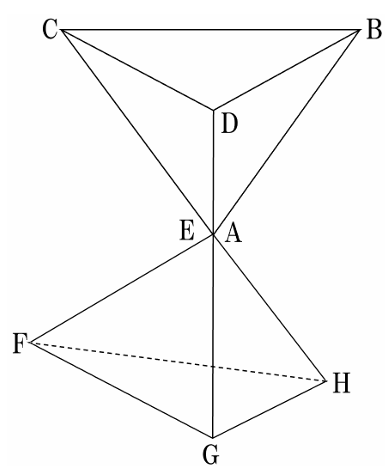
\includegraphics[width=5cm]{fig_1999_3.png}
\end{flushright}

\newpage

\begin{flushleft}
{\huge 4}
　$xyz$空間において$xy$平面上に円板$A$があり$xz$平面上に円板$B$があって以下の2条件を満たしているものとする．
\begin{description}
\item[(a)]$A$，$B$は原点からの距離が1以下の領域に含まれる．
\item[(b)]$A$，$B$は一点$P$のみを共有し，$P$はそれぞれの円周上にある．
\end{description}
　このような円板$A$と$B$の半径の和の最大値を求めよ．
ただし，円板とは円の内部と円周をあわせたものを意味する．
\end{flushleft}

\newpage

\begin{flushleft}
{\huge 5}
\begin{description}
\item[(1)]$k$を自然数とする．
$m$を$m=2^k$とおくとき，
$0<n<m$を満たすすべての整数$n$について，
二項係数${}_mC_n$は偶数であることを示せ．
\item[(2)]以下の条件を満たす自然数$m$をすべて求めよ．
\begin{center}
条件：$0 \leqq n \leqq m$を満たすすべての整数$n$について二項係数${}_mC_n$は奇数である．
\end{center}
\end{description}
\end{flushleft}

\newpage

\begin{flushleft}
{\huge 6}
　$\displaystyle\int_0^\pi e^x {\sin}^2x dx>8$であることを示せ．
ただし，$\pi=3.14\cdots$は円周率，$e=2.71\cdots$は自然対数の底である．
\end{flushleft}

\end{document}
